
\begin{textblock*}{3cm}(8.8cm,0.6cm) % {width}(x, y)
   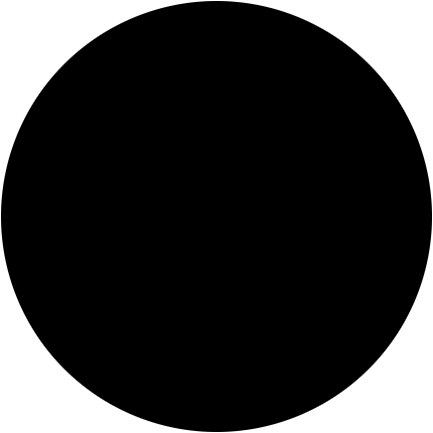
\includegraphics[width=1.0cm]{./bilder/cirkel.png}
\end{textblock*}

\vspace*{-8mm}
Borra ett hål här i pärmen för att fästa din penna: %{\Huge $\bullet$}

\subsubsection*{Konsten att sjunga!}
Att sjunga är verkligen något av det roligaste som finns\dots

Morris Thånell BME19 och Elin Helmersson E21\\
Sångbokskommittén 2024



\newpage

Tack till de som hjälpt oss med boken...

\dots

\newpage

% % Save current headsep
% \newlength{\oldheadsep}
% \setlength{\oldheadsep}{\headsep}

% % Reduce headsep and set pagestyle
% \newpage
% \setlength{\headsep}{0pt}
% % \thispagestyle{noheader}

% \newgeometry{top=10pt, bottom=30pt, left=30pt, right=30pt}
% \setlength{\footskip}{15pt} % Decrease to move the footer up



\vspace*{-13mm} % Pull the content upwards (adjust as needed)
\enlargethispage{15mm} % Allow more vertical space at the bottom



% \enlargethispage{1.5cm}  % Adjust as needed

\begin{center}
    \textbf{Viktig information}
\end{center}


\begin{textblock*}{6cm}(6.0cm,1.5cm) % {block width}(x-coordinate, y-coordinate)
  
\includegraphics[width=3.5cm]{./bilder/profilbild_stor.png} % Adjust the image size as needed
\end{textblock*}
\vspace*{3.0mm}
\begin{parse lines}[\noindent]{#1\\\vspace{0.5mm}}
  Ägare:\vspace{2mm}
  Program:\vspace{2mm}
  Inskrivningsår:\vspace{2mm}
  Födelsedatum:\vspace{2mm}
  Telefonnummer:\vspace{2mm}


  Lämna tillbaka mig till den här adressen:\vspace{8mm}
  Hittelön:
  Jag vill reinkarneras som:
  I mitt förra liv var jag:
  Detta dricker jag helst:
  Bästa barndomsminnet:
  Julklappen jag aldrig fick:
  Mest impulsiva jag gjort:
  Om jag hade en superkraft:
  Bästa partytrick:
  Favoritintegral:
  Min säng är så här bred:
  Första kändis-crush:
  Gör så här för att charma mig:
  Om jag hade fått välja nollningstema:
\end{parse lines}

\newpage
% \subsubsection*{Innehållsförteckning}
\clearpage
\tableofcontents
\thispagestyle{plainnohead}



\newpage

\begin{center}
  \vspace*{1.5cm}
  {\fontsize{20}{20}\textbf{Vett och etikett}}\\
  \vspace{0.7cm}
  {\fontsize{12}{12}\textit{Om den pryde själv får välja}}
\end{center}
\addtocwithheader{Vett och etikett}  % Add entry to TOC and set header
\noBackground
\newpage
\resetBackground

\subsection*{Klädkod}
För att underlätta förmedlingen av vem som ska ha på sig vad använder vi oss av följande namn.\\

\textbf{Truls}: Manlig teknolog\\
\textbf{Trula}: Kvinnlig teknolog\\
\textbf{Trelsa}: För hen som inte vill identifiera sig med någon av ovanstående.

\subsubsection*{Högtidsdräkt - Militäruniform och folkdräkt}

\textbf{Truls}: Militäruniform, folkdräkt eller frack\\
\textbf{Trula}: Militäruniform, folkdräkt eller balklädding\\
\textbf{Trelsa}: Se Truls/Trula

\subsubsection*{Civil högtidsdräkt}

\textbf{Truls}: Frack, vit skjorta, vit fluga\\
\textbf{Trula}: Balklädding\\
\textbf{Trelsa}: Se Truls/Trula

\subsubsection*{Smoking}
\textbf{Truls}: Smoking, vit skjorta, svart fluga\\
\textbf{Trula}: Lång klänning, dock behöver den inte vara lika elegant som en Balklädding. Tänk festligt.\\
\textbf{Trelsa}: Se Truls/Trula

\subsubsection*{Mörk kostym}
\textbf{Truls}: Mörkblå, mörkgrå eller svart kostym. Vit skjorta med sidenslips eller fluga i valfri färg.\\
\textbf{Trula}: En finare känning, men även byxdress elelr halvlång kjol med jacka går bra.\\
\textbf{Trelsa}: Se Truls/Trula

\subsubsection*{Kavaj}
Ibland även kallad bruten elelr udda kavaj.\\
\textbf{Truls}: Kavaj och ett par finare byxor (dock inte kostymbyxor), skjorta i valfri färg. Fluga eller slips kan vara trevligt!\\
\textbf{Trula}: Cocktailklänning, kjol eller dress.\\
\textbf{Trelsa}: Se Truls/Trula

\subsubsection*{Ouverall}
\textbf{Truls}: Ouvve\\
\textbf{Trula}: Ouvve\\
\textbf{Trelsa}: Se Truls/Trula
\\
\\
\\
\subsection*{Elektroslajd}
Ta på dig ouvven.\\
Släng dig ner för backen.\\
Gör ouvven fin.

\newpage

\subsection*{Mer om teknologens utstyrsel}
Det kan trots föregående sidors fenomenala utlägg ibland kanske vara lite förvirrande att avgöra vad man ska ha på sig.
Men något som alltid går hem i Teknlogsammanhang är självfallet Teknologmössan. 
Denna kan och bör man bära oavsett tillställning.
\\


Teknologmössan får dock enbart pryda de teknologer som med någorlunda bravur genomfört Nollningen på TLTH.
Och likt fjällräven med sin vinterpäls och sommarpäls är det av största vikt att även Teknologen skiftar mellan sin vita sommarmössa och sin mörkblåa vintermössa.
Men till skillnad från fjällräven så finns det för teknologen väldefinierade datum för när den ena eller den andra mössan ska användas.
\\


\textbf{Sommarmössa: 1:a maj - 3:e oktober}


\textbf{Vintermössa: 4:e oktober - 30:e april}
\\


Viktigt att notera är dock att oavsett årstid så används den vita sommarmössan då Högtidsdräkt bärs.
\\


För att lättare hålla koll på vilka datum som gäller bör man inte jämföra med vilka datum som det är tillåtet att ha dubbdäck på sin bil, för det är bara nästan samma datum.


\newpage
\enlargethispage*{1cm}

\subsection*{Plösen}
Som den observante noterat är teknologmössan berikad med en tygflik som hänger ned på mössans högra sida, denna flik kallas för plös. 
\\

\subsection*{Spegaten}
Från plösen hänger ett tofsprytt snöre försynt och dinglar. På detta snöre fäster man efter varje påbörjat läsår en spegat. En vit spegat för de som studerar Elektroteknik och en rödvit spegat för de som studerar Medicin och Teknik.
Det finns även en svart som indikerar sabattsår, en skogsgrön för ett år i lumpen och en vit-blå-silver som visar att man spenderat ett år som heltidare i Teknologkårens tjänst.
\\


\subsection*{Tofsen}
Utöver att hålla rätt antal spegater på rätt plats är det av yttersta vikt att själva tofsen håller sig fin. Ett bra sätt att säkerställa detta på är knyta en knut längst ner på alla tofsens hundratals trådar. Om en annan individ gör detta slitgöra åt dig, borde det så klart belönas med en fin puss!


Är man i förhållande och inte känner för att pussa en massa folk kan man göra en knut av själva snöret ovanför spegaterna för att signalera detta.
\\


\vissteduatt{Visste du att mer information om teknologmössan går att hitta \\
 på KFS hemsida?}
\newpage

\subsection*{Vid bordet}
Han har sin bordsdam till höger om sig och hon har sin bordsherre till vänster.
Herren drar ut stolen till höger för att hjälpa sin bordsdam till bords eller från bordet.
\\

Damens väska hängs i första hand över stolsryggen, armstödet eller damens axel.
Alternativt kan väskan placeras mellan ryggen och stolsryggen eller i knäet.
Den serverade maten får inte påbörjas utan värdens tillåtelse.
Vid större sittningar uppmanar en bra värd de sittande att äta direkt av rätter som skall förtäras varma.
Innan maten har påbörjats får man dricka av vattenglaset samt bryta och äta eventuellt bröd som serverats.
\\

Ditt vattenglas är alltid placerat längst till höger, sedan används glasen från höger till vänster i takt med att rätterna påbörjas.
Värden bestämmer när en rätt påbörjas.
Servetten du får till bords skall placeras i knäet innan först rätten påbörjas. Den skall placeras på stolen då du lämnar bordet innan sittningens slut, absolut inte på bordet.
Vid sittningens sult läggs servetten upp på vänsersidan av tallriken, lätt skrynklad.
\\

\newpage

Besticken används i ordningen "utifrån och in".
Besticken till förrätten ligger således ytterst.
Vid rätter som kräver sked så ligger skeden på höger sida om tallriken, förrutom vid dessert.
Alla dessertbestick finns ovanför tallriken.
Om det ligger en gaffel till höger sida om tallriken så betyder det att rätten enbart äts med gaffel.
Besticken får inte placeras lutande mellan bordet och tallriken, utan esticken förblir på tallriken när de har börjat användas. 
Då besticken ät placerade på tallriken som klockslaget tjugo i fyra betyder det att du fortfarande äter,
medan klockslaget tjugo över fyra betyder att du är klar.
\\

Vid bal och finare sittningar är det brukligt att ha med sig en present till sin bordsgranne. 
En fun fact är att begreppet "vänterprassla" kommer just från att det fanns/finns vissa herrar som inte kunde/kan hålla sig till sin bordsdam, 
utan istället såg/ser sig om till vänster for att prova lyckan där.

\vissteduatt{Visste du att bordsherre och bordsdam är bordsplaceringsbenämningar
\\ som avser att underlätta sittningsförfarande och är helt könsneutrala?}
\newpage

\subsection*{Skålen}

När det skålas och det ska skålas korrekt så börjar man 
med att skåla med sin bordsgranne, sedan med din sekundära 
bordsgranne och slutligen rakt över till den mittemot. 
Efter dricker man ur och upprepar denna process, fast baklänges.
\\

Alltså:
Han börjar till höger,

sedan vänster och slutligen rakt fram.

Hon börjar till vänster,

sedan höger och slutligen rakt fram.

Drick, sedan alltsammans baklänges.

\vissteduatt{\colorbox{yellow}{En myt säger att man får börja äta av maten vid fler gäster än\\
åtta vid bordet, detta är fel!}}

\newpage

\subsection*{Underhållning}
På sittningar bjuds det utöver mat och dryck (som man förvisso betalt för) oftast även på underhållning.
Denna kan yttra sig antingen som sång från Sångförmännen eller i form av ett spex.
Till dessa akter finns det ett par förhållningsregler att beakta.
\\

1. När Sångförmännen talar, är man tyst.\\
2. När Sångförmännen sjunger, sjunger man med.\\
3. När Sångförmännen drar ett skämt, skrattar man.\\
4. När det är spex, är man tyst.\\
5. Punkt 4 får brytas om spexet är så roligt att man behöver skratta. Då skrattar man.\\
6. Har man varit på toaletter väntar man till spexet är fördigt innan man sätter sig till bords igen.\\
7. Behöver man gå på toaletten under ett spex - bad luck.\\
8. Vill man spexa på en sittning anmäler man det i god tid till Sångförmännen.\\
9. Spontansång beivras!\\
10. Spontansång uppmuntras om Sångförmännen meddelat satt sången är fri. Då gäller inte Punkt 9.\\
11. Tempo är okej om Sångförmännen sagt att det är det.\\
12. Tempo är inte okej om Sångförmännen sagt att det inte är det.\\
13. Har sångförmännen inte sagt något om Tempo lär de göra det snart.\\
\\


\newpage

Efter ett spex visar de sittande sin uppskattning genom att be spexarna att spexa en gång till.
Detta görs genom att sjunga nedanstående sång, som initieras av Sångförmännen.
\\

\begin{parse lines}[\noindent]{\textit{#1}\\}
  Det där det gjorde han/hon/de fan så bra, hej!
  En skål uti botten för honom/henne/dem nu vi ta
  Och alla så dricka vi nu [namn på spexare/spexarna eller mumlande] till 
\end{parse lines}

Den sista raden upprepas till det att spexaren eller spexarna svarar:
\\

\begin{parse lines}[\noindent]{\textit{#1}\\}
  Och namn på spexare/spexarna spexar gärna en gång till.
\end{parse lines}

Efter det andra spexet är det dock färdigspexat, men självfallet ska de sittande 
ändå ännu en gång visa sin uppskattning genom en sång, som även den initieras av Sångförmännen.
\\

\subsection*{Ettans gutår}
\begin{parse lines}[\noindent]{#1\\}
  Det var i vår ungdoms fagraste vår
  Vi drack varandra till och vi sade Gutår
\end{parse lines}


\newpage


% \subsubsection*{Hur man är på sittning}
% \subsubsection*{REGLER}

% \subsubsection*{Mellanskål}
% OBS! En mellanskål initieras alltid av sångförmännen.

% Nu är det dags för mellanskål
% Om det så är det sista jag gör
% Nu är det dags för mellanskål
% Hoppas inte föräldrarna stör
% Nu är det slut på versen 
% Det är dags för mellanskål

% \newpage

% \subsection*{Hur man tågar}

% När ett stort antal teknologer behöver förflytta sig till fots, kan detta göras genom att tåga. 
% När man möter ett övergångsställe stannar delar av tåget med jämna mellanrum för att låta bilar passera.
% När man tågar håller man sig åt sidan av vägen där man går så att cyklar och andra kan åka förbi.

% När man tågar ska man såklart sjunga, och här passar E-sektionens kampvisor mycket väl.

% En annan låt som gärna sjunges är den här under. 

% Oh ale ale
% a riki tiki tamba
% a massa massa massa
% baloe baloe baloe
% I said baloe baloe baloe

% Eller den här:

% ||: Har ni mjölkat alla kossorna idag
% Ja, vi har mjölkat alla kossorna idag :||

% Mjölka kossa får du glass annars får du ananas
% Ale, ale, ale, ale
% Mjölka kossa, ale, ale

% Andra sidan är ni klara?
% Har ni erat glada barnasinne kvar?

% \newpage

\subsection*{Ordförande}
Ordförande har till uppgift att leda och representera sektionen och en massa andra saker. 
Detta är dock inte alls lika viktigt om man ställer det mot förväntningarna som finns på Ordförande när han/hon/hen sjunger Taggig Blomma! 
Man får aldrig låna ut sin sångbok till Ordförande när denne skall sjunga Taggig Blomma ty då får man aldrig se den igen.
\\

\vspace{1cm}

\subsection*{Taggig Blomma} 
\index[alfa]{Taggig Blomma}
\index[anfa]{När man söker LTH att glömma...}
\songinfo{Mel: Rosen \\Text: Jan Grenner F71}

\begin{parse lines}[\noindent]{#1\\}
  När man söker LTH att glömma,
  är det skönt att glaset sitt få tömma
  Glömma att alla studier gått på sne’
  och att tentamen gick åt helvete

  För just nu idag, så köpte jag
  en liter sprit och min börs den var tom
  Renat så klart, det var underbart
  att få tömma den i min gom
  
\end{parse lines}

\newpage

\begin{parse lines}[\noindent]{#1\\}
  När jag som vanligt gick till bolaget
  för att bota mina abstinensbesvär
  så svarade dom helt enkelt: "Nej,
  det skall nog inte vara mera här
  Ni är ju full och för ung
  Har ni legitimation?
  Utan den får ni minsann ingen flytande muntration"
  
  Men ingenting kunde hindra mig
  jag måste ha gök ikväll
  På stan jag drev tills en langare jag såg
  i bil av senaste modell
  Flaskan blänkte, kapsylen blixtrade i dess topp
  Darrhänt jag tänkte:
  "De' va' faan va' korken va' svår att få opp!"
  
  När man söker...
  
\end{parse lines}

\newpage

\subsection*{Några ord om akademisk kvart - 2}

{\fontsize{9}{9}\selectfont 
Förr i världen på den tid då bilar och varmvattenberedare
fortfarande hörde till ovanligheterna, var det svårt för studenterna 
att hålla koll på tiden. Anledningen till detta var att det fanns en
stor brist på klockor, fickur och mobiltelefoner.
\\

I både Lund och Uppsala, emellertid, var man bortskämda 
med stora domkyrkor med klockor som slog varje hel timme.
När man hörde klockan slå, visste man således att det var
dags att bege sig mot föreläsningen. Men självfallet tog det
ju en liten stund att ta sig till föreläsningssalen och detta
resulterade i införandet av den akademiska kvarten.
\\

Traditionsbundna och morgontrötta som vi studenter
är, så lever fenomenet kvar än idag. Står att en
föreläsning börjar kl. 8, betyder det därmed att den
egentligen börjar kl. 8:15.
\\

För att krångla till det ytterligare så finns även något 
som kallas akademisk dubbelkvart. Detta infaller på
helgdag och kvällstid, d.v.s efter kl. 18:00. I princip 
gäller samma regler som för den enkla akademiska kvarten,
men det är en halvtimmes fördröjning istället. En sittning
som börjar kl. 19 börjar alltså i själva verket kl. 19:30.
\\

Om man någon gång däremot SKA komma på
exakt på klockslaget och akademisk kvart
INTE ska tillämpas markeras detta med ordet "prick" eller (.).
Efter kl. 18 skriver man "prick prick" eller (..).
\\

\colorbox{yellow}{skriva om 4 siffror? Kåren gör det och vi gjorde det förut, 
med det står med 4 siffror i time-edit och LU nämner det inte}
}

\newpage


\subsection*{Social for Dummies}
När man är på en sittning är det viktigt att man är social med sina bordsgrannar. 
Ofta är det så att man inte känner någon bordsgranne sen tidigare och vid sådana 
fall kan det vara lite svårt att vara social. Därför har Social for Dummies 
skapats för att lätta på spänningen.
\\

För att kunna vara social så måste man kunna kommunicera med dem i sin omgivning. 
Detta görs enklast oralt. Förutom att introducera sig och fråga bordsgrannarna vad de 
heter och pluggar kommer nu några bra samtalsämnen samt frågor.
\\
\begin{itemize}[itemsep=0.0em]
  \item Dagens konjunkturläge
  \item Microsoft vs. Apple vs. Linux?
  \item Vädret. Finns det inget väder, prata om tryck.
  \item Politiska läget på Island?
  \item Kan björnar klättra?
  \item Det stoltaste du gjort i trä– eller syslöjden?
  \item Vad hade du jobbat som om du var utomjording?
  \item Vad är det galnaste du gjort?
\end{itemize}


Skulle det vara så att din bordsgranne är något av en s.k. Gamer, så finns följande sida för sådana.

Reglerna för \textit{Luffarschack} kan förhoppningsvis Gamern.

OBS! Använd gärna blyerts!

\newpage

\thispagestyle{plainnohead}

\phantom{osynlig text}

\begin{textblock*}{3cm}(1.0cm,1.0cm) % {width}(x, y)
   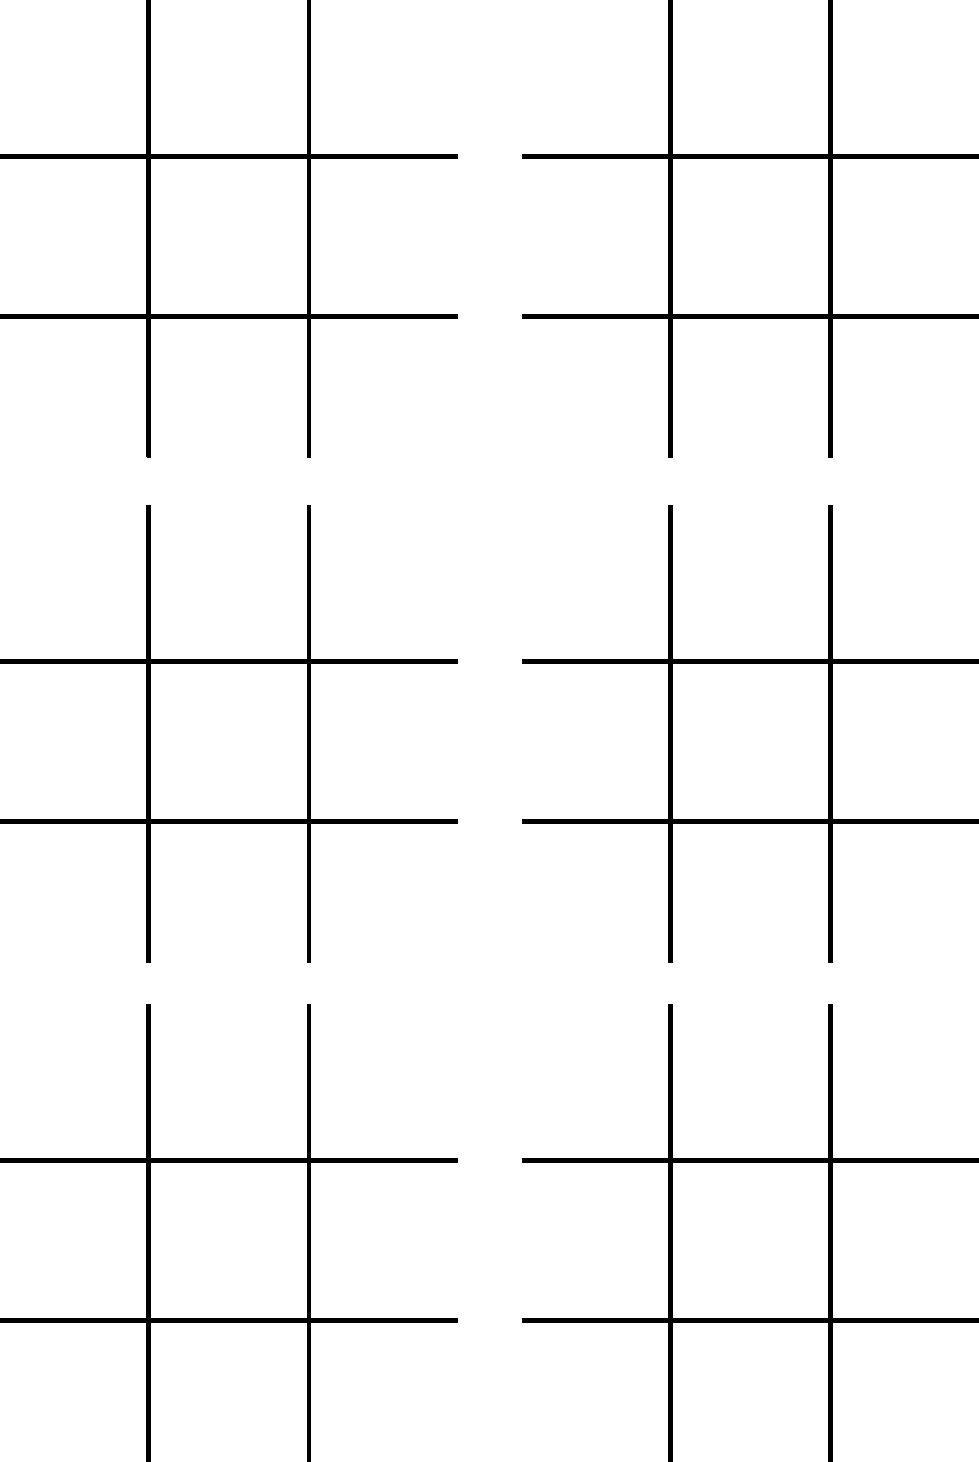
\includegraphics[width=8.5cm]{./bilder/luffarschack.png}
\end{textblock*}


\noBackground

\newpage
\resetBackground

\thispagestyle{plainnohead}

\vspace*{-13mm} % Pull the content upwards
\enlargethispage{15mm} % Allow more vertical space at the bottom

\begin{center}
    \normalfont\normalsize\bfseries Bordsgranne of Fame
\end{center}

Namn: \hspace{2.5cm} Sittning: 

% \newpage
% \setlength{\topskip}{0pt}  % Remove the top skip
\vspace*{0.3cm}
\rule{\textwidth}{0.0mm}
\vspace*{0.65cm}
\rule{\textwidth}{0.4mm}
\vspace*{0.65cm}
\rule{\textwidth}{0.4mm}
\vspace*{0.65cm}
\rule{\textwidth}{0.4mm}
\vspace*{0.65cm}
\rule{\textwidth}{0.4mm}
\vspace*{0.65cm}
\rule{\textwidth}{0.4mm}
\vspace*{0.65cm}
\rule{\textwidth}{0.4mm}
\vspace*{0.65cm}
\rule{\textwidth}{0.4mm}
\vspace*{0.65cm}
\rule{\textwidth}{0.4mm}
\vspace*{0.65cm}
\rule{\textwidth}{0.4mm}
\vspace*{0.65cm}
\rule{\textwidth}{0.4mm}
\vspace*{0.65cm}
\rule{\textwidth}{0.4mm}

\noBackground

\newpage
\resetBackground




\subsubsection*{Tankar på vad vi vill lägga till}

\subsubsection*{Mellanskål}
Ibland när man sjunger en väldigt lång låt (se The Engineer's Drinking Song) kan det vara så att man behöver vattna strupen under låtens gång. Såklart vill man inte behöva missa en vers bara för att man behöver dricka. Då kan man mellan två verser sjunga låten nedan för att få utbringa en skål, innan man fortsätter sjunga igen.

\subsection*{Mellanskål} 
\index[alfa]{Mellanskål}
\index[anfa]{Mellanskål}
\songinfo{Mel: Fredagsmys}

\begin{parse lines}[\noindent]{#1\\}
    Det dags för mellanskål
    Om det så är det sista jag gör
    Snart är det mellanskål
    Hoppas inte föräldrarna stör
    Nu är det slut på versen 
    Det är dags för mellanskål
\end{parse lines}


\subsection*{Hur man tågar}

När ett stort antal teknologer behöver förflytta sig till fots, kan detta göras genom att tåga. 
När man möter ett övergångsställe stannar delar av tåget med jämna mellanrum för att låta bilar passera.
När man tågar håller man sig åt sidan av vägen där man går så att cyklar och andra kan åka förbi.

När man tågar ska man såklart sjunga, och här passar E-sektionens kampvisor mycket väl.

En annan låt som gärna sjunges är den här under. 

Oh ale ale
a riki tiki tamba
a massa massa massa
baloe baloe baloe
I said baloe baloe baloe


\subsubsection*{Dubbelkolla att det är andra upplagan}
Hör av oss till förra Sångbokskommittén och fråga om detta är andra upplagan. Vad fanns innan detta?


\newpage
\subsection*{Rita dig själv}

% \begin{textblock*}{6cm}(4cm,5.0cm) % {block width}(x-coordinate, y-coordinate)
%   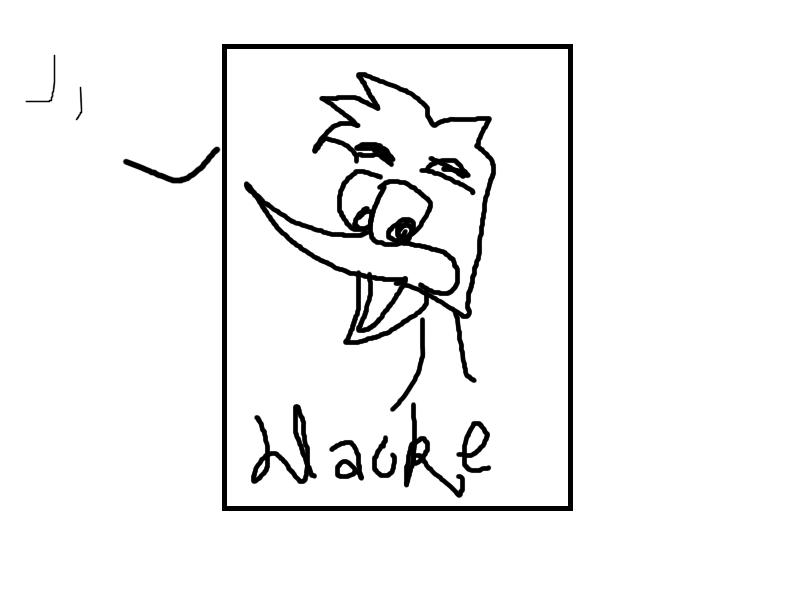
\includegraphics[width=5.5cm]{./bilder/Untitled.png} % Adjust the image size as needed
% \end{textblock*}

Gör som Hacke och rita dig själv i någon annans bok!

\begin{textblock*}{6cm}(1.55cm,3.45cm) % {block width}(x-coordinate, y-coordinate)
  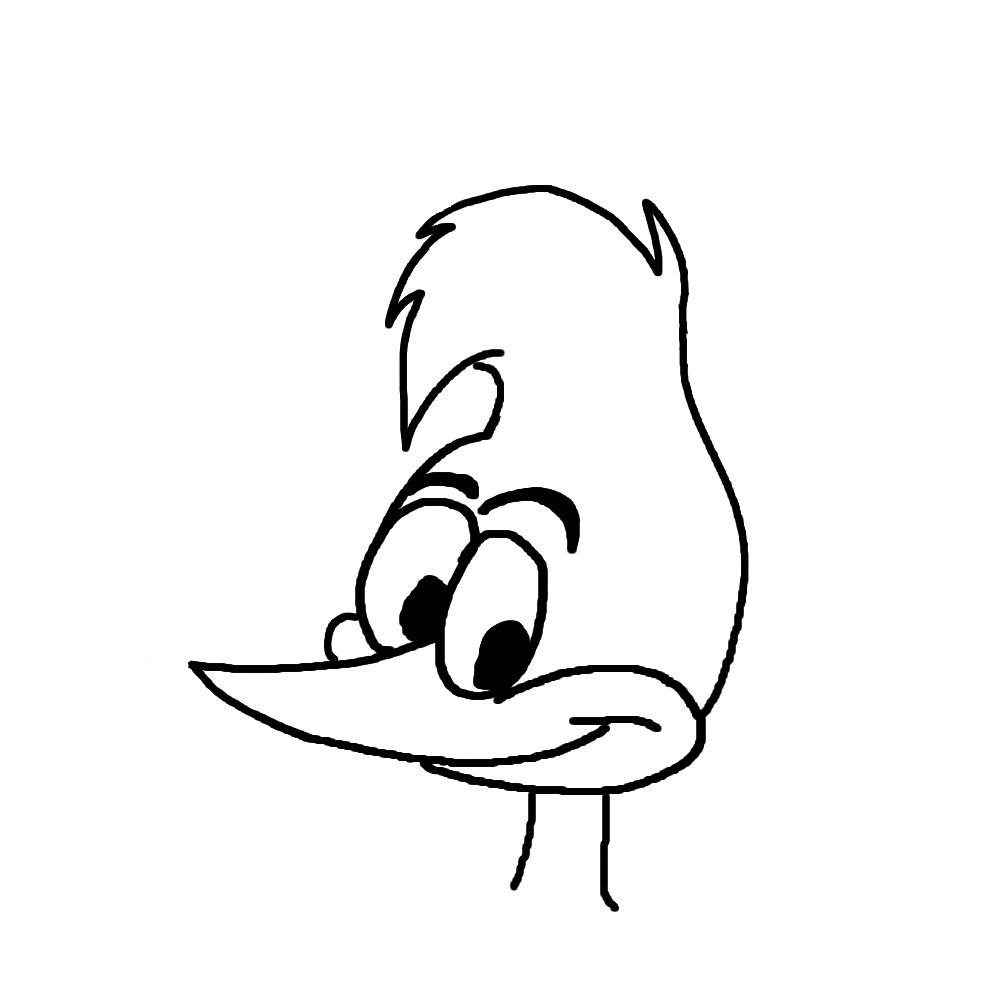
\includegraphics[width=2 cm]{./bilder/ramar/hacke_portratt_2.png} % Adjust the image size as needed
\end{textblock*}



\begin{textblock*}{6cm}(1cm,2.7cm) % {block width}(x-coordinate, y-coordinate)
  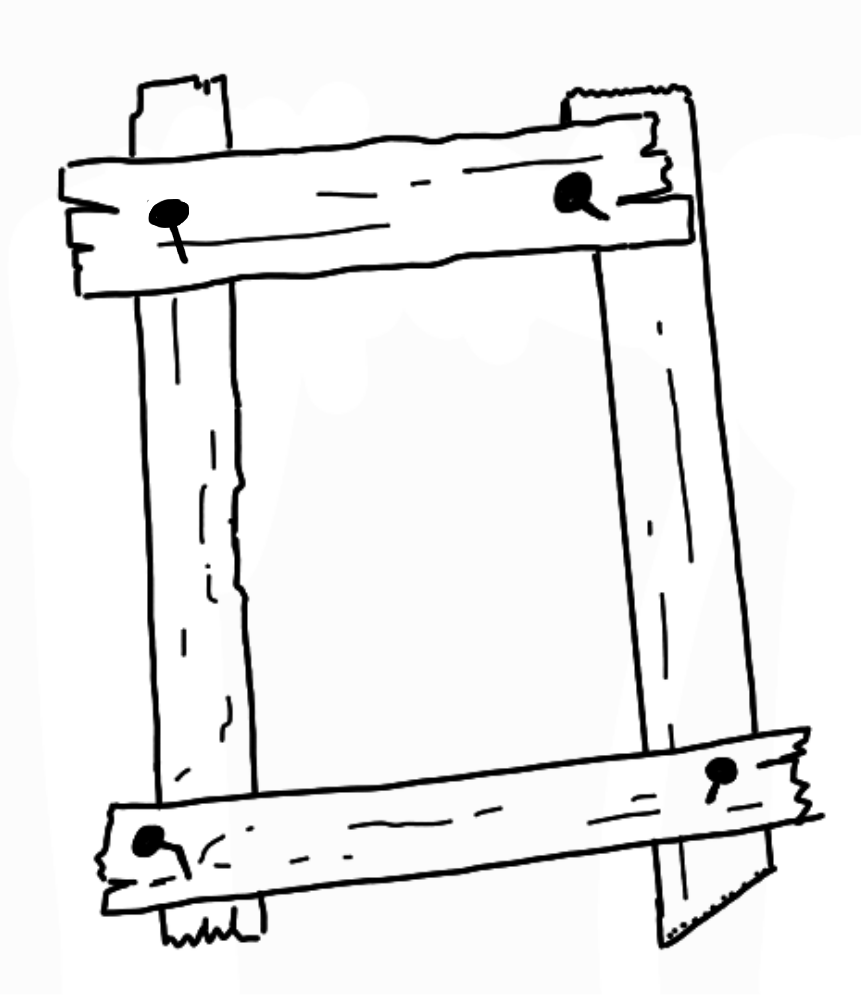
\includegraphics[width=3cm]{./bilder/ramar/Ram4.png} % Adjust the image size as needed
\end{textblock*}

\begin{textblock*}{6cm}(4cm,2.7cm) % {block width}(x-coordinate, y-coordinate)
  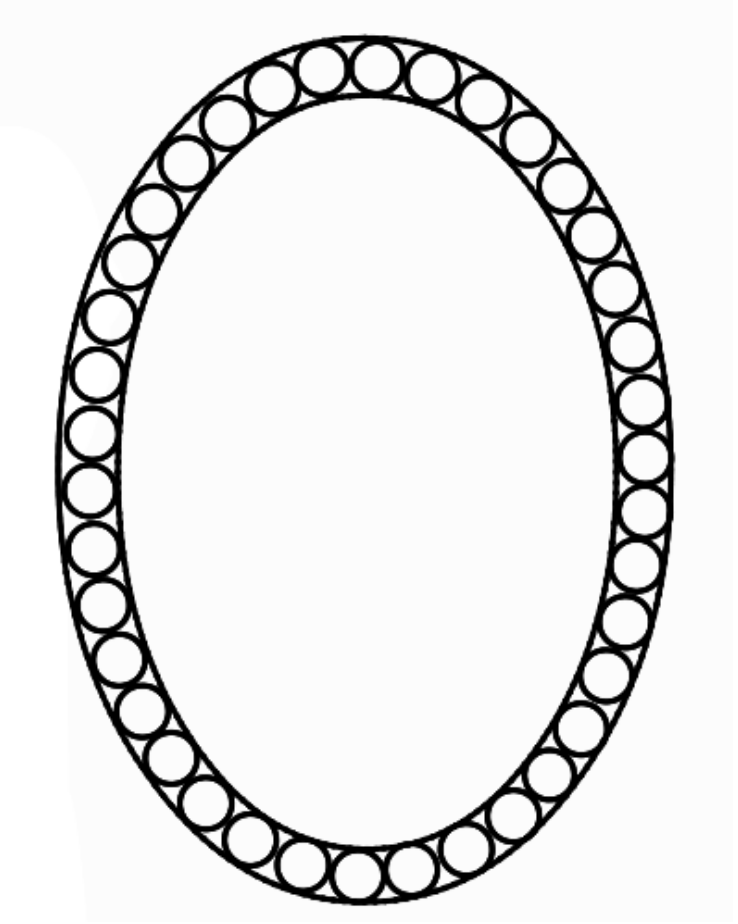
\includegraphics[width=2.6cm]{./bilder/ramar/Ram5.png} % Adjust the image size as needed
\end{textblock*}

\begin{textblock*}{6cm}(6.6cm,3.2cm) % {block width}(x-coordinate, y-coordinate)
  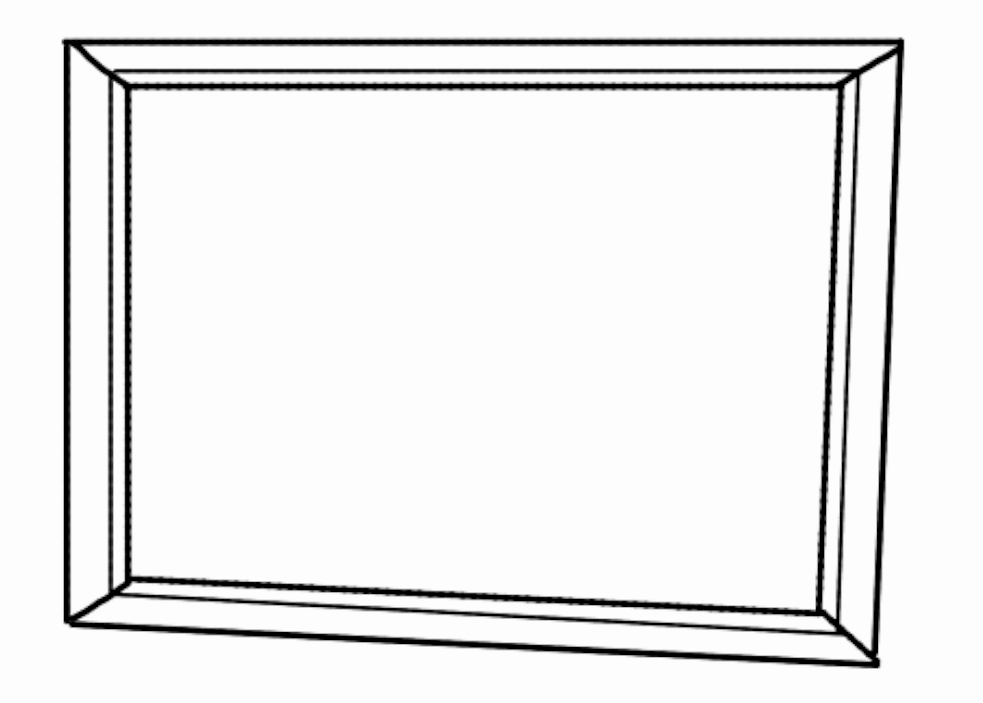
\includegraphics[width=3.5cm]{./bilder/ramar/Ram6.png} % Adjust the image size as needed
\end{textblock*}



\begin{textblock*}{6cm}(0.8cm,6.4cm) % {block width}(x-coordinate, y-coordinate)
  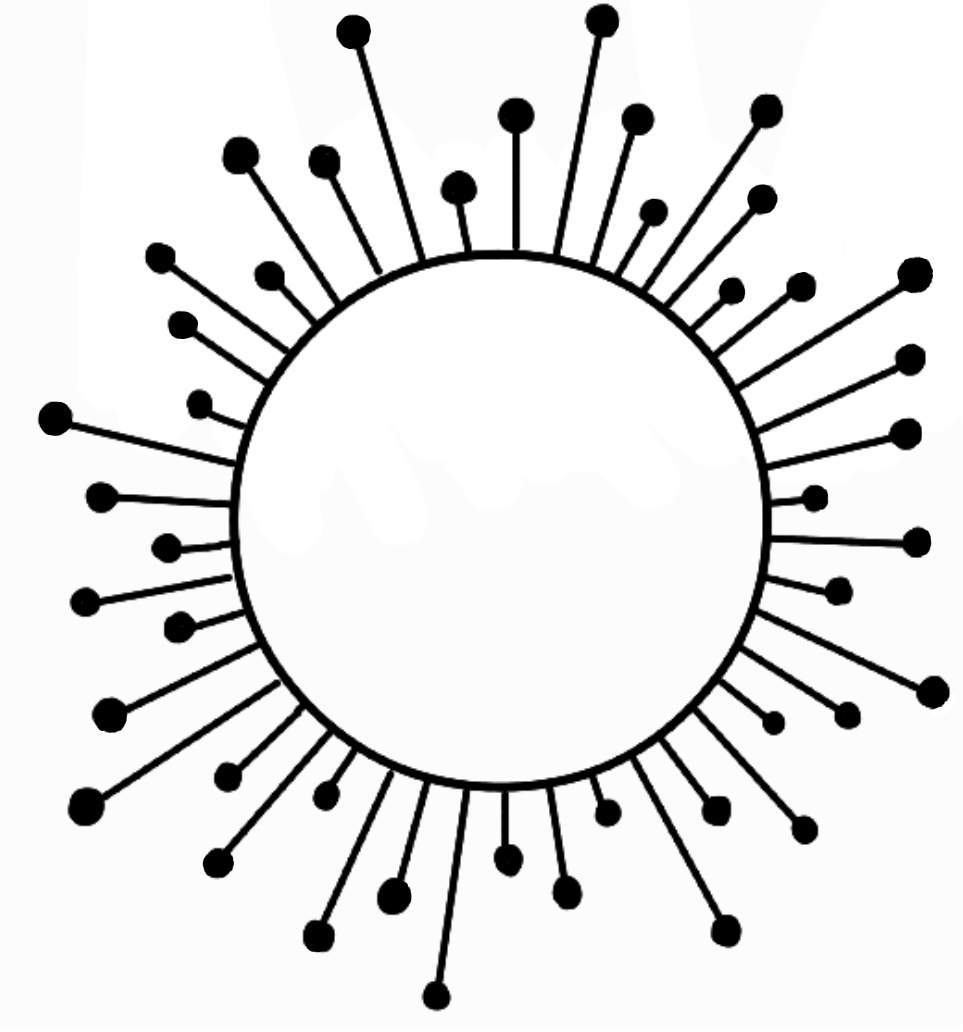
\includegraphics[width=3.3cm]{./bilder/ramar/Ram7.png} % Adjust the image size as needed
\end{textblock*}

\begin{textblock*}{6cm}(4.2cm,6.2cm) % {block width}(x-coordinate, y-coordinate)
  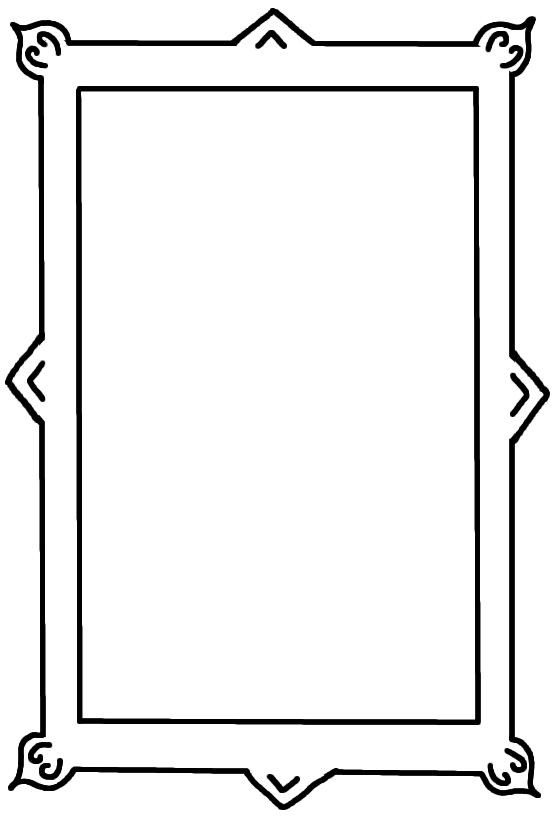
\includegraphics[width=2.5cm]{./bilder/ramar/ram1.png} % Adjust the image size as needed
\end{textblock*}

\begin{textblock*}{6cm}(6.9cm,6cm) % {block width}(x-coordinate, y-coordinate)
  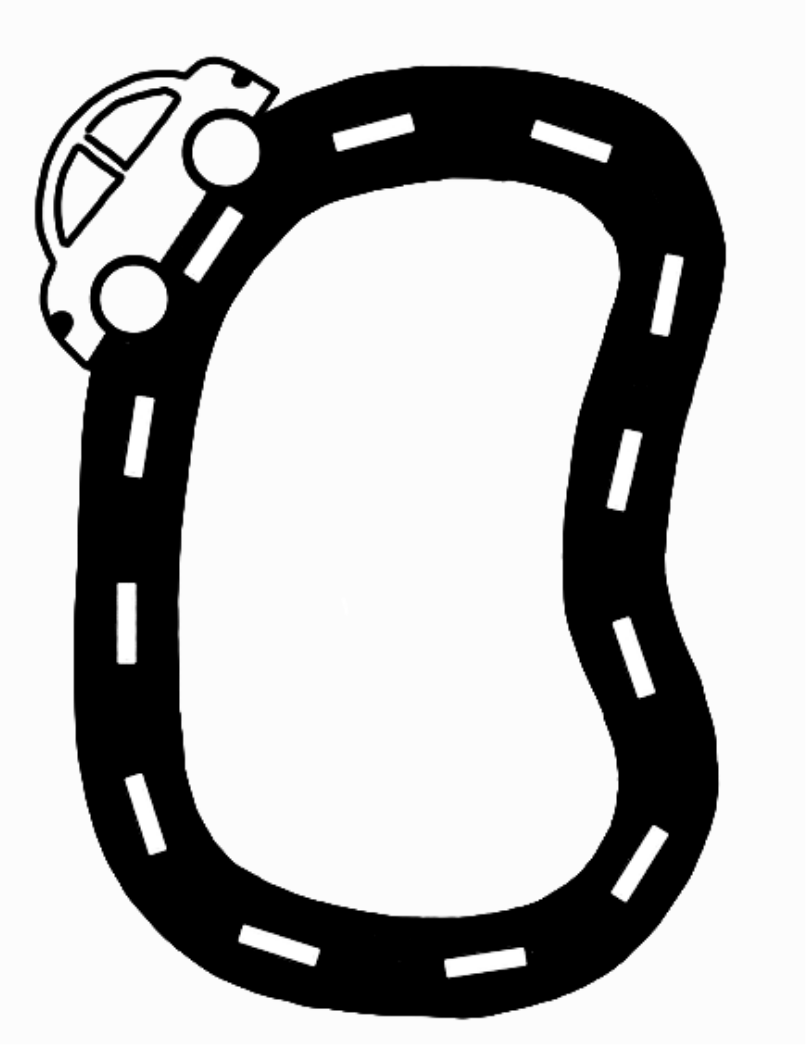
\includegraphics[width=2.8cm]{./bilder/ramar/Ram8.png} % Adjust the image size as needed
\end{textblock*}



\begin{textblock*}{6cm}(1.1cm,10.3cm) % {block width}(x-coordinate, y-coordinate)
  \includegraphics[angle=-90, width=3.2cm]{./bilder/ramar/Ram3.png} % Adjust the image size as needed
\end{textblock*}

\begin{textblock*}{6cm}(4.4cm,10.1cm) % {block width}(x-coordinate, y-coordinate)
  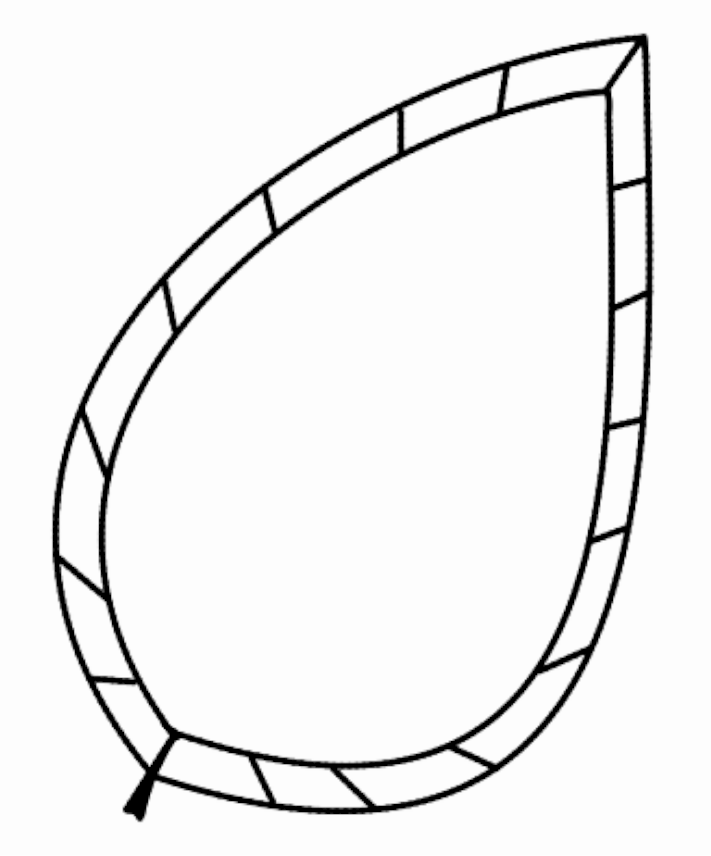
\includegraphics[width=2.6cm]{./bilder/ramar/Ram9.png} % Adjust the image size as needed
\end{textblock*}

\begin{textblock*}{6cm}(7.1cm,9.8cm) % {block width}(x-coordinate, y-coordinate)
  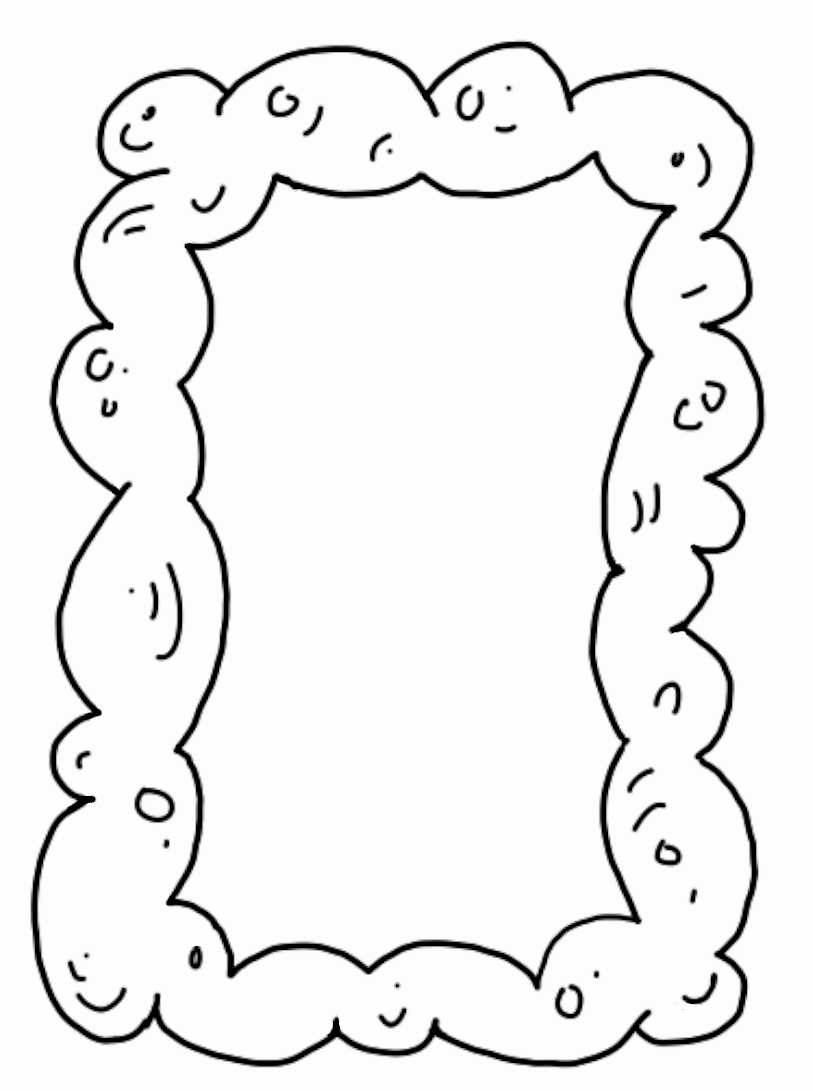
\includegraphics[width=2.8cm]{./bilder/ramar/Ram10.png} % Adjust the image size as needed
\end{textblock*}

\newpage

% tom sida

% \newpage